\chapter{Traffic scheduling}
\label{chap:gf}

Internet is growing -> people depend more and more on it - its harder to maintain QoS.

 QoS - that is bandwidth allocation (fairness for all, because clients share some limits), acceptable delay(jitter)
 
ISP - klienti si platia za nejaku kvalitu

co je to traffic scheduling - stoji medzi 2-3 layer OSI, mby trosku HW popisat? netdevice queue vs queing discipline 

\section{Bufferbloat}
\label{chap:bb}

In gateways of packet-switched networks, short-term differences between arrival and departure rate naturally happen. To balance these bursts, buffers are used --- packets are waiting in queues until they can be sent towards their destination. This helps avoiding outgoing link starvation and increases throughput. Without buffers, the gateway has no place to store incoming packets and they get dropped, which decrease throughput.


However, the more packets are in a queue, the longer packets stay in it and the longer it takes to be delivered. Unfortunately, queues in modern networks tend to fill up and stay 'bloated' \cite{Gettys:2012:BDB:2063176.2063196}. That means some amount of packets always stay in the queue (it never becomes empty), even if there are no incoming bursts to balance.

\begin{figure}
	\centering

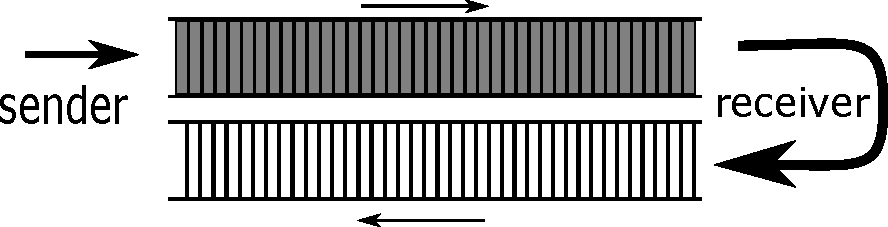
\includegraphics[width=137mm]{drawings/tcp_no_bottleneck}
\caption{TCP without bottleneck. The grey rectangles are packets. Horizontal dimension is time, vertical is bandwidth. That means the area of rectangle is size of packet.}

\label{fig01:no_bottle}
\end{figure}

To understand why queues become bloated, let's take a look at Transport Control Protocol (TCP), which is the most widely used layer 4 protocol. It achieves its reliability with following policy: After packet is transmitted, receiver sends an ACK packet back to sender to let him know which packets have been successfully received, and which must be resent. But waiting on ACK after each packet would provide miserable throughput and most of the time both sides would wait on single packet. The sender goes ahead and transmit packets without getting ACKs on previous ones. This fills the whole route, so at all times one packet is being sent, one packet is being received. The ACKs that are coming back retain the same spacing. The situation is displayed on Figure \ref{fig01:no_bottle}.

Figure \ref{fig01:no_bottle} shows connection with constant bandwidth along whole path, which is rarely the case in today's Internet. Typical path consists of many hops with links of different bandwidth. That means somewhere must be a bottleneck - link with lowest bandwidth. If the sender transmitted at the rate of adjacent link, the network would become congested. Bottleneck link would not be able to forward all incoming traffic, its buffer would fill, and the rest of arriving packets would be dropped. That actually induces even more traffic, because sender would try to resend dropped packets.


%tcp by potrebovalo vediet aky badwidth ma bottleneck
TCP must limit upstream rate. In ideal case, it would work at the rate of slowest link. However, the sender does not have any information about bottleneck whatsoever. TCP uses congestion window: it is amount of bytes TCP can send without receiving an ACK. When an ACK is received, it frees space in congestion window, and next packet can be sent, filling the window again. The first ACK is received after round trip time (RTT) - the time it takes to transmit packet on path sender-receiver-sender.

To maximize throughput, size of congestion window should be at least the (bottleneck) bandwidth-delay product (product of bandwidth and RTT) bytes. In this case, the sender fills the pipe with packets just before it receives first ACK and is allowed to send following packets. On the other hand, if congestion window exceeds the bandwidth-delay product, the excessive packets stay in queues along the path and cause delay. 

%TCP uses slow start algorithm to find ideal congestion window at start, and then congestion control algorithm takes over to maintain it near the inflection point of maximized throughput and minimizing delay. This if solution to avoiding congestion collapse, but the Internet encounters problem of persistently full buffers - bufferbloat.



Bufferbloat is caused by mismatch between congestion window and actual RTT \cite{CoDel}. In reality, estimating the window size is difficult. Always-changing network load affect both RTT and bandwidth, paths change thanks to rerouteing. Buffers can really only be measured at the bottleneck and even there it is hard to differentiate between useful and useless buffers that only cause delay.

\begin{figure}
	\centering
	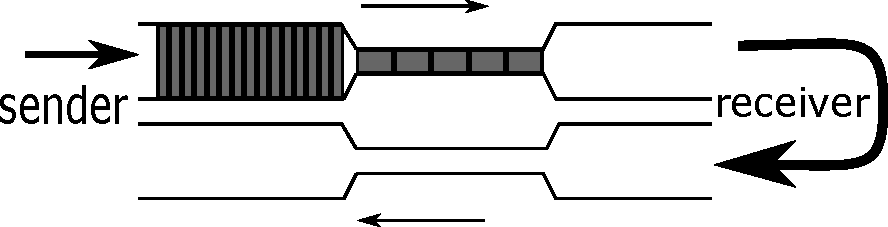
\includegraphics[width=137mm]{drawings/tcp_bottleneck_1}
	\caption{Start of TCP communication.}
	
	\label{fig02:bottle_1}
\end{figure}


Figure \ref{fig02:bottle_1} shows a starting TCP communication. Illustrated network consists of 3 subnetworks. The left and right have bandwidth 30 Mb/s, the middle one has 10 Mb/s. One packet has 30kb. TCP Congestion window is 20 packets. The sender starts by transmitting whole window of packets back to back. They arrive at edge of bottleneck network and get enqueued there, because of bandwidth difference. A packet arrives from left network every 1 ms, but only every 3 ms is one dequeued. On the right side, they retain spacing given by bottleneck as shown in Figure \ref{fig03:bottle_2}. The receiver turns incoming packets into ACKs with the same spacing. The sender then sends one packet of data for each ACK it gets.

This way, after one RTT, whole connection has gotten into state of equilibrium. The bottleneck is fully utilized, so the throughput is as high as possible. However, a queue at the middle network will never be empty. At first, it had to hold the burst of whole congestion window. Once all 20 packets were sent, 14 of them were waiting in the queue, 6 had already been forwarded to middle network. Then, no packets were enqueued and every 3 ms one was dequeued. Until one RTT passed, first ACK was delivered and next packet sent into left network. After that, every 3 ms one packet arrives and one leaves. 5 packets stay there and every one of them waits long 15 milliseconds. Also, they block buffer space other connections could use. 

\begin{figure}
	\centering
	\includegraphics[width=137mm]{drawings/tcp_bottleneck_2}
	\caption{TCP after one RTT}
	
	\label{fig03:bottle_2}
\end{figure}

The queue stayed in the buffer in figure  \ref{fig03:bottle_2} because congestion window was set to 5 more packets than the bandwidth-delay product. Determining the size is not an easy task. At start of TCP, slow start algorithm \cite{Jacobson:1988:CAC:52324.52356} is used to determine size of congestion window. It grows exponentially, increasing size of window with each ACK received, until a threshold is reached or packet is dropped.  After that, congestion avoidance takes over to maintain it. Over the years of TCP in service, many variants were introduced. Currently CUBIC [ref] is used widely. 

%emhasize that it is a way to communicate
Congestion windows are managed by TCP endpoints, while congestion and bufferbloat takes place in gateways along the path. There is no direct communication channel between them. When the buffer becomes full, the next packets must be dropped simply because there is no room for them. When TCP does not receive an ACK, it the congestion avoidance algorithm reduces the window and slows down.

Relatively new is Explicit Congesion Notification (ECN) \cite{rfc3168:ECN}. There are 2 bits reserved for ECN in IP header, so packets may be marked, that there is ongoing congestion. Both sides have to support ECN  - the receiver has to read the 2 bits and send ACK with the same bits back. The sender then may react like ACK didn't arrive at all. In May 2017, passive support for ECN was available on 70 \% of popular websites \cite{ECN:proceedings}.

This all indicated, that simple tail drop queues, which drop packets only when they are full may be superseded by more sophisticated queues right in the gateways. It involves the counter-intuitive idea of dropping perfectly good packets even if buffer is not full yet. But it indicates a problem, while still having room for balancing bursts. This approach is called Active Queue Management (AQM), and is recommended to use throughout the Internet.


\subsection{RED}

%kde sa nachadza queue management?

\begin{figure}
	\centering
	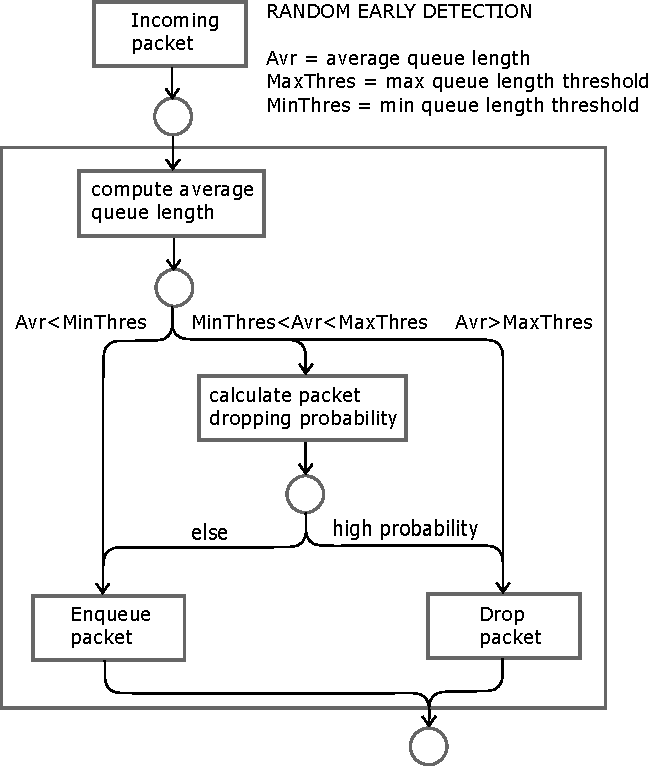
\includegraphics[width=137mm]{drawings/RED}
	\caption{The Random Early Drop algorithm  (Image taken from wikipedia \cite{RED:picture}) }
	
	\label{fig04:RED}
\end{figure}

In 1993, Sally Floyd and Van Jacobson introduced Random Early Drop (RED) \cite{Floyd:1993:RED:169931.169935}. It monitored average length of queue. According to it, it may drop (mark) incoming packet with certain (possibly 100 \%) probability, which is function of average. It addressed congestion avoidance problem as well as TCP synchronization problem, that were encountered using tail drop. However, it had quite a few parameters, which have to be set differently in various networks. Without this tuning, it functioned poorly which led to general reluctance of deployment, although it was recommended by Internet Engineering Task Force \cite{rfc2309} in 1998.

To determine the average, RED uses exponential weighted moving average:
\[
avg := (1 - w_q)avg+w_qq.
\]
$q$ is number of packets in queue and $w_q$ is parameter of RED that represents degree of weighting decrease, or how much the average responds to new packets and how much weight have the past states. Too high $w_q$ would mean bias against short bursts. With lower $w_q$, average is more fluid and queue responds to congestion slower.

At each enqueue, the $avg$ is compared to two parameters $min_{th}$ and $max_{th}$, as showed on Figure \ref{fig04:RED}. If it lower than $min_{th}$, packet is just enqueued as is. If $avg$ is higher than $max_{th}$, the packet is marked (dropped). This ensures, that if endpoints respond to marking properly, or packets are actually dropped, number of packets in queue will not exceed maximum for long.

If $avg$ is between the thresholds $min_{th}$ and $max_{th}$, packet is marked (dropped) with probability $p_a$, that is function of the average and . Let $p_b$ be linear function of $avg$ that varies from 0 to $max_p$ ($max_p$ is parameter of RED):
\[
  p_b = max_p \frac{(avg - min_{th})}{max_{th} - min_{th}}.
\]
Further, the final marking probability $p_a$ depends on when was the last packet marked (dropped):
\[
p_a = \frac{p_b}{1-count \cdot p_b},
\]
where $count$ is number of packets that were enqueued since the last mark (drop). This ensures, that dropped packets will never be too far, nor too close \cite[Section 7]{Floyd:1993:RED:169931.169935}.

RED also has option to work based on number of bytes in buffer instead number of packets. In this case:
\[
  p_b = max_p \frac{(avg - min_{th})}{max_{th} - min_{th}}
\]\[
  p_b = p_b \frac{size_{packet}}{size_{max}}
\]\[
  p_a = \frac{p_b}{1-count \cdot p_b},
\]
where $size_{packet}$ is size of packet being enqueued and $size_{max}$ is maximum size of packet. This way, large packets are more likely to get marked, and probability corresponds more precisely to actual time that packet spend in queue.

%!!!!!!!!!!!!!!!!!!je v pohode tam dat takyto odstavec o ktorom neviem vela??
Over the years, several variants of RED have been introduced. With Weighted RED different packets have different probability functions for different classes of traffic (classified for example by DSCP). Adaptive RED \cite{Floyd01adaptivered:} tunes the RED algorithm to remove sensitivity to some of the parameters. Robust RED \cite{RRED} was proposed to counter low-rate Denial-of-Service attacks.

\subsection{CoDel}

In 2012, Jacobson and Nichols introduced Controlled Delay - CoDel \cite{CoDel}. Their AQM uses local minimum length of queue as indication of bufferbloat. Additionally, it works only with sojourn time - the time packet spends in queue. That means it is independent of bandwidths of adjacent links, because it only works with time - if it is deployed in a backbone, with 10 Gb/s bandwidth, acceptable queue will be 50 Mb big. On the other hand on slow links, say 10 Mb/s, corresponding acceptable buffer is only 50 kb. CoDel measures time packets spend in queue and if it exceeds a threshold for a longer time, it starts to drop packets.

It has 2 parameters:
\begin{itemize}
	\item $Target$ is the target delay CoDel tries to keep. Defaults at 5 ms.
	\item $Interval$ sets period of time for which it is OK exceed $Target$. Defaults at 100 ms.
\end{itemize}
So CoDel drops packets, if packets spend more than $Target$ time in queue for more than $Interval$ time. Also, CoDel does not drop packets, if fewer that MTU (Maximum Transmission Unit) worth of bytes is in queue.

Every time a packet arrives, a time stamp is tagged to it. At dequeue, CoDel looks how long was the dequeued packet in queue. If packets have exceeded the $Target$ time for at least $Interval$, CoDel enters dropping state. In this state, packets are dropped at an increasing rate until the sojourn time of packets at front is lower than $Target$. The next drop time is calculated as follows:
\[
  DropInterval = \frac{Interval}{\sqrt{count}},
\]
where count is number of packets dropped since dropping state entry and DropInterval is time after next packet will be dropped.


\section{Fair queueing}

Research shows that simple first-come, first-serve (FCFS) scheduling does not treat all network users fairly in all situations. In many cases, we want to ensure that every user of network is provided with the same quality of service. Further, it is beneficial if scheduling separates well and ill-behaved users, so that only the latter experience consequences of their behaviour. Set of algorithms that enable this is attributed fair queueing.

In many of the proposed solutions, fairness is achieved by adding firewalls between different streams of packets traversing network, or flows. We use definition from \cite{Zhang:1990:VCN:99517.99525}. A flow has two properties:
\begin{itemize}
	\item A flow is a stream of packets that traverses the same route from the source to the destination and requires the	same grade of service at each router or gateway in the path.
	\item In addition, every packet can be uniquely assigned to a flow using prespecified fields in the packet header.
\end{itemize}
 
\begin{figure}
	\centering
	\includegraphics[width=137mm]{drawings/parking_lot}
	\caption{The parking lot problem.}
	
	\label{fig05:ParkingLot}
\end{figure}

One of issues addressed by fair queueing is parking lot problem. Typically, routers accomplish some amount of fairness by giving fair access to traffic coming on different input links. However, this approach is not fair to all \textit{users}. Consider network displayed in Figure \ref{fig05:ParkingLot}. Gateway G1 treats both flows F1 and F2 equally, thus both flows occupy half of link G1-G2. G2 does the same, it gives half of the bandwidth to flow 3 and second half to the traffic from link G1-G2. However, from perspective of flows, F1 and F2 have only 1/4 of the bandwidth while F3 has half of the bandwidth. In the outcoming link of G3, situation is the same and F1 only has one 1/8 of the bandwidth. In other words, portion of bandwidth allocated to flow drops exponentially with number of hops it must get through.

Second issue is connected to behavior of users themselves. In gateways working on FCFS basis, misbehaving user that sends more traffic than others, and does not slow down on packet drops, may actually get bigger portion of bandwidth than well behaving users. Consider a router with several users connected on LAN, one of them is ill-behaved generates traffic that by itself exceeds routers out--link. The rest of users detect congestion and slow down, resulting in leaving even bigger proportion of the bandwidth to the bad user. Furthermore, delay discussed in section \ref{chap:bb} is shared among all users and if one bloats the buffer, the others experience consequences too.

Nagle \cite{Nagle:FQ} proposed to use one FCFS queue per one flow encountered by the gateway. At enqueue, router finds the right queue based on IP header. Queues are dequeued in a round-robin fashion --- the queues take turns in fixed order. There is a list of all queues and at each dequeue gateway transmits the first packet of the first queue in the list. Then, the first queue is taken from the front and put in the back of the list.

%flow stealing

This solves both of mentioned problems, maintaining separate queue for each flow requires that the gateway to be able to map from flow identifiactor (for example source-destination address pair, ports and protocol may be considered too) to corresponding queue at each dequeue. This can be easily implemented in $O(log n)$, where n is number of queues, however that is not fast enough for simple routers with ever-rising bandwidths. McKenney discusses several possible implementations in \cite[Section 2]{SFQ}.

Nagle's original algorithm has yet another flaw --- it doesn't take packet size into consideration. Demers et al. devised an ideal algorithm called bit-by-bit round-robin (BR) \cite{demers1989analysis} addressing the flaw. It simulates that each queue sends one bit at a time in round-robin fashion. Based on this simulation, it computes time $t$ whole packet would leave its queue. Then, BR inserts the packet in a queue sorted by $t$. Unfortunately, the best known algorithms that insert into sorted queue require $O(log n)$ time, where n is number of flows (since at most one packet from each flow needs to be in the priority queue at the same time).

Although the Nagle's FQ algorithm was perfected to be truly fair, it requires too much resources. Following algorithms have O(1) complexity, while being only slightly less fair.


\subsection{Stochastic Fairness Queueing}
%aspon jednu figure bud z FQ alebo SFQ?

SFQ was proposed by McKenney \cite{SFQ} to address the inefficiencies of Nagle’s algorithm. It uses hashing to determine the flow each packet belongs to. Although one would normally require one queue for every flow and thus use hashing with chaining, McKenney suggests using considerably less queues and allow collistion. This guarantees $O(1)$ queue determination. The disadvantage is that some flows may collide, end up in the same queue and thus be treated unfairly. However, if the number of queues is sufficiently larger than the number of active flows, probability of unfairness is low.
Tu further beat this disadvantage, SFQ changes the hashing periodically (e.g. every 10 seconds) by varying salt of hash function.

SFQ services queues in round-robin fashion, without taking packet lengths into consideration, so it is unfair, if average packet size vary in different flows.

SFQ uses bufferstealing: When there is no more space in the buffer, a packet is dropped from the queue with the highest number of packet instead of dropping packet being enqueued. To implement this in O(1), McKenney suggests bucket sorting technique: there is an array $A$ indexed by number of packets. In $i$-th field of the array, there is a list of all queues that contain $A[i]$ packets.

McKenney's scheme is valuable for bufferstealing and stochastic approach, however does nothing about unfairness caused by flows having different size of packets.

\subsection{Deficit round-robin}

Deficit round robin \cite{EffDRR} is an algorithm that extends SFQ and takes packet length into consideration, so every flow gets the same bandwidth in the long term regardless of its packet characteristics. It still requires only $O(1)$ time for all operations.

Enqueue is done in the SFQ--way: DRR chooses queue based on hash of certain IP header fields. It keeps list of active queues and works in $O(1)$. When the buffer is full, packet is dropped from the fullest queue instead of dropping the incoming one.

%popisat najskor Q_i co znamenaju, povedat ze je to viac general schema, no da sa pouzit aj na fair q
The novelty of DRR lies in modified round-robin. For each flow, DRR needs quantum $Q_i$ as parameter: it is the number of bytes that can be sent each round from flow $i$. Further, there is a state variables $DC_i$ for each flow. At each round, DRR sends at most $DC_i + Q_i$ bytes. Once sending next packet would break this rule, queue is put at the back of active queues list and $DC_i$ is set to amount of remaining bytes:
\[
  DC_i = DC_i + Q_i - b_{sent},
\]
where $b_{sent}$ is number of bytes sent that round from queue i. If there are no packets in queue left, it is deactivated instead of putting it in the back.

\begin{algorithm}
	\caption{DRR dequeue}
	\label{alg01:DRR_deq}
	\begin{algorithmic}
		\While{true}
			\State F $\leftarrow$ pop(ActiveQueues);
			\If {empty(F)}
				\State Deactivate(F)
			\ElsIf{F.DC \textgreater~head(F).PacketSize}
				
					\State {F.DC $\leftarrow$ F.DC - head(F).PacketSize}
					\State \Return pop(F)
			\Else \Comment{The packet is bigger than DC}
				\State F.DC $\leftarrow$ F.DC + Q
				\State push(ActiveQueues, F)
			\EndIf
		\EndWhile
	\end{algorithmic}
\end{algorithm}
%                                                                                 vvvv only if all Q_i are same
Although DRR may not send exactly the same amount of bytes each round, it becomes fair  over several rounds time, because every round,  all that remains in $DC_i$ from the previous round transfers to the next. Thus, any unfairness caused by atomicity of packets are smoothed over time.

%analyza??

\subsection{FQ CoDel}

\begin{figure}
	\centering
	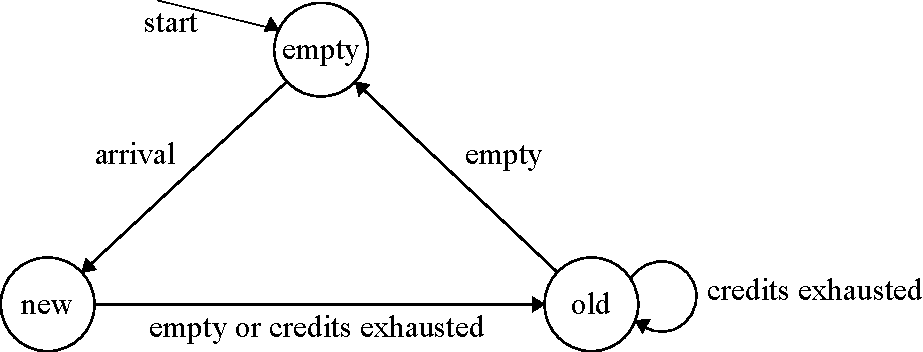
\includegraphics[width=137mm]{drawings/fq_codel}
	\caption{FQ CoDel state-machine}
	
	\label{fig06:fqcodel}
\end{figure}


Flow Queue Control Delay \cite{fq_codel} is traffic scheduler combines ideas of SFQ and DRR with bufferbloat battling capability of CoDel. It uses modified DRR and replaces FCFS queues for flows with CoDel queues. Currently, several linux distributions as well as systemd use FQ CoDel as default root traffic control.

FQ CoDel processes flow in the DRR fashion, however it divides active queues into two groups: new and old. The new ones are prioritized: packet is never dequeued from an old flow, if list of new queues is not empty. Empty queue becomes new, when a packet comes to it. New queue becomes old (it is pushed at the back of old flows list), if it becomes empty, or its DC (credits) is exhausted. Old queue becomes empty, if there are no packets left in it. So every flow has its life cycle in this order: it is first empty, then new, old and empty again. The state machine is illustrated in figure \ref{fig06:fqcodel}.

FQ CoDel has parameters $Target$ and $Interval$ that configure the underlying CoDels. Further, there is $Quantum$, that is parallel of DRR's $Q_i$, however $Quantum$ applies to all queues. Instead of $DC$, amount of resources is called credits. $Limit$ is maximum number of packets the scheduler can hold at the same time.

When a packet is enqueued in FQ CoDel, its flow is found based on its IP header. Then, CoDel takes it over - it is timestamped and put in the back. If the flow was empty, it is pushed back into the list of new queues and its credits are set to $Quantum$.

To protect buffer from overload, FQ CoDel keeps track of total packets it is holding. Since a packet has just been enqueued, $Limit$ may be exceeded. If it is, the algorithm finds queue with the largest byte count and drops 64 packets from the \textit{front}. Dropping several packets at once amortises the time needed to find the longest queue.

The algorithm does most of the work at dequeue. First, it has to choose flow $F$ to dequeue packet from --- either head of new queues list, or head of old queues list, if new one is empty. If $F$ has negative credits, it means at least $Quantum$ bytes have already been served, and FQ CoDel pushes it in the back of old queues list and starts over witch choosing $F$.

Second, it dequeues next packet from CoDel of flow $F$. Two things may happen:
\begin{enumerate}
	\item CoDel drops all packets on dequeue --- change state of the flow based on Figure \ref{fig06:fqcodel} and start over.
	\item CoDel returns a packet --- subtract the size of packets from credits of flow $F$ and send the packet away.
\end{enumerate}

\section{Bandwidth allocation}

-TBF - HFSC

\section{Differentiated services}
-classes of traffic
?

